Kimodo-Policy adapts Kimodo's pretrained motion prior for visually grounded, closed-loop humanoid control. We describe its root--body--hand architecture and visual conditioning (Sec.~\ref{sec:method_architecture}), motion-prior transfer and history-conditioned control (Sec.~\ref{sec:t2m_transfer}), and training and inference (Sec.~\ref{sec:training_inference}). Background on Kimodo and ControlNet is provided in Appendix~\ref{sec:preliminaries}.

\begin{figure}[H]
  \centering
  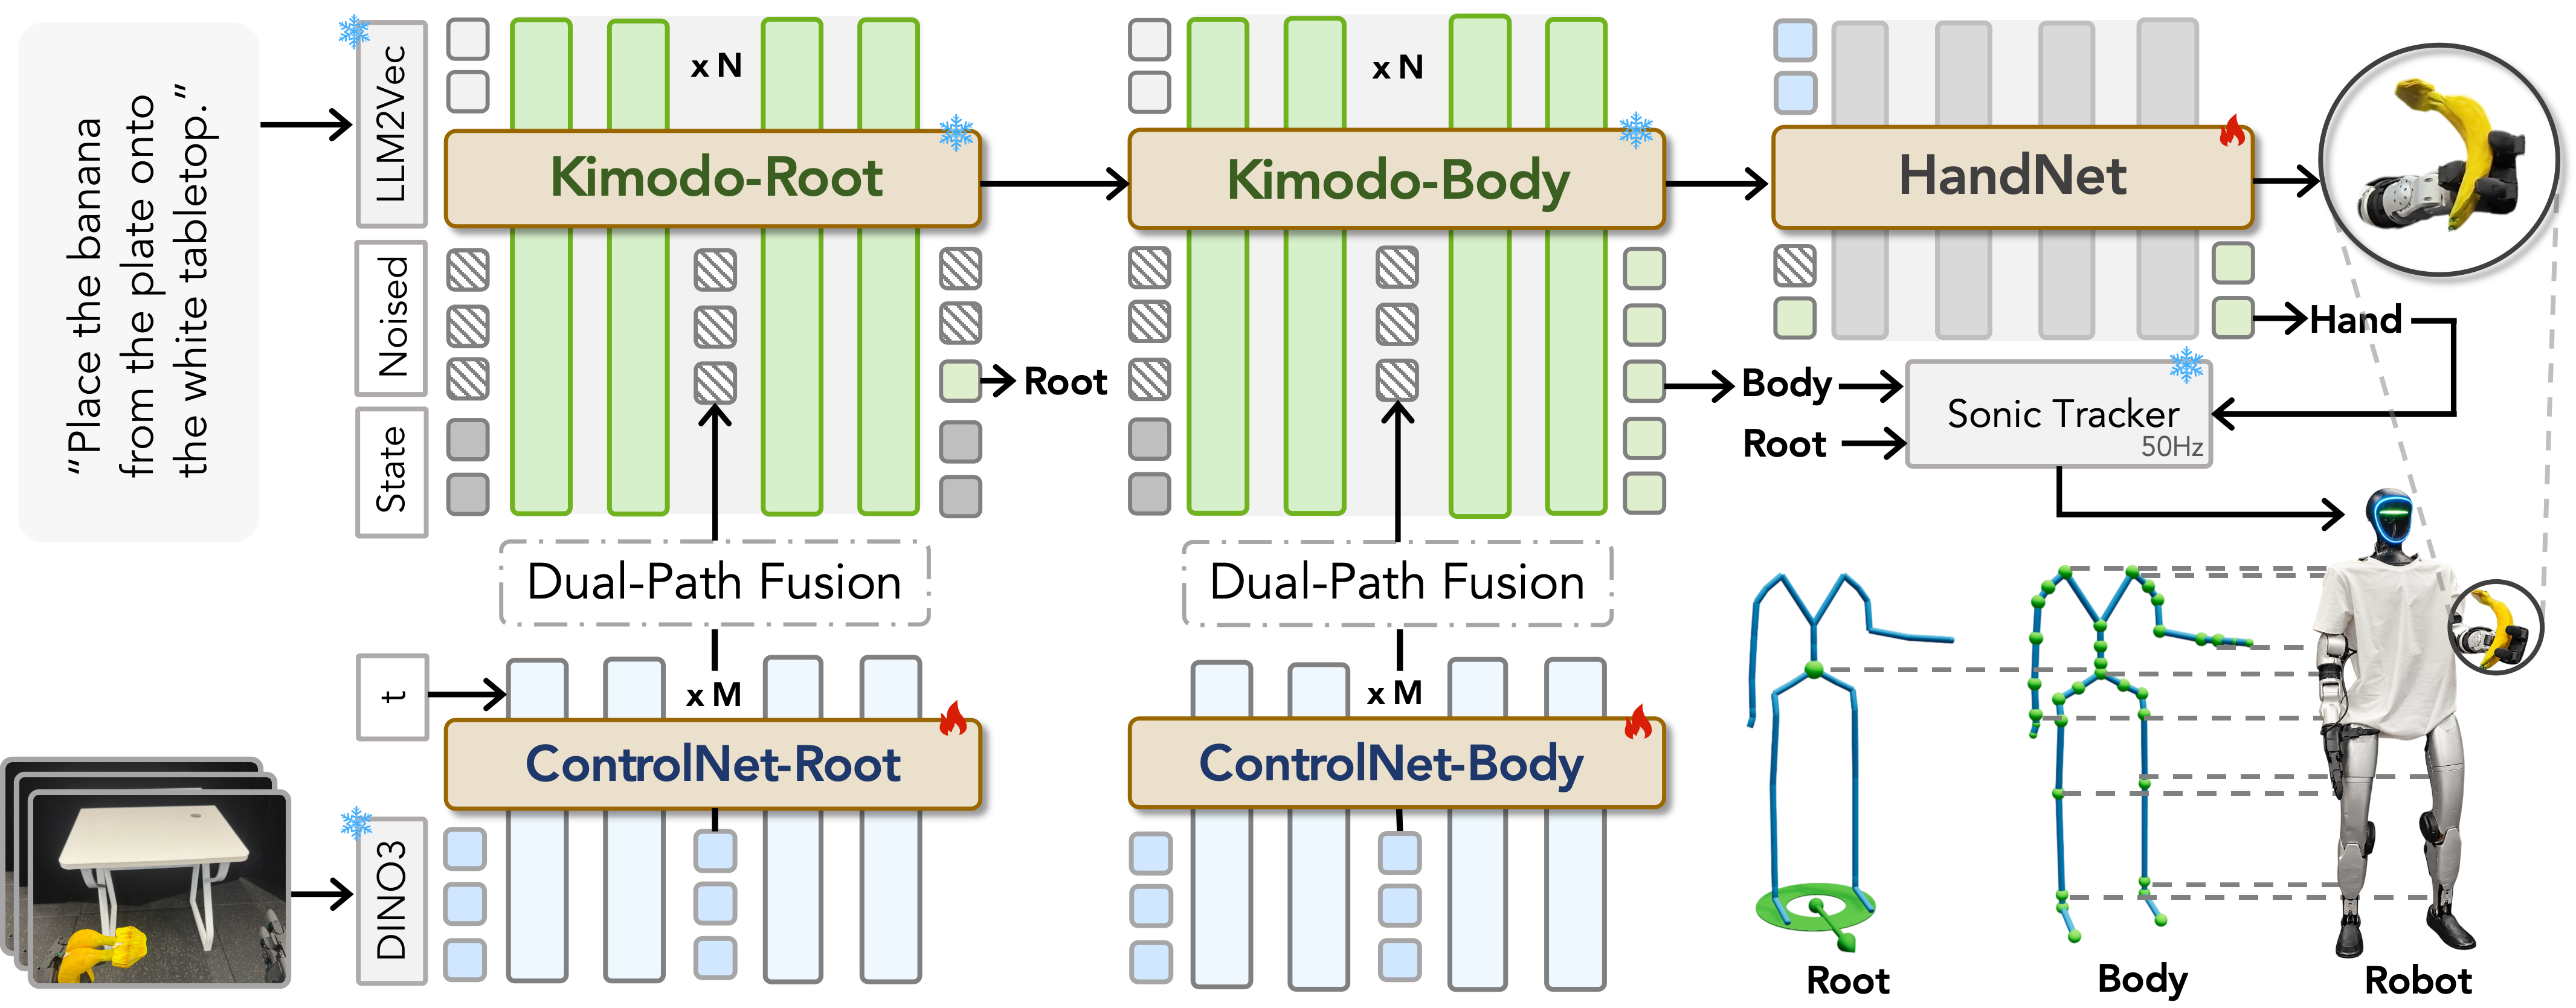
\includegraphics[width=\textwidth]{image/method.png}
  \caption{\textbf{Kimodo-Policy architecture.} Colored blocks: \inlinecolorblock{green!55!black}{green!15} Kimodo denoisers, \inlinecolorblock{blue!55!black}{blue!10} DINOv3-conditioned~\cite{dinov3} ControlNet, and \inlinecolorblock{gray!65}{gray!15} HandNet. Dashed boxes show Dual-Path Fusion: motion-query cross-attention and spatial-to-temporal MLPs. Root predictions condition body generation; future body features guide bilateral hand control. The Motion Projector maps root--body outputs to tracker references. Snowflakes/flames mark frozen/trainable modules.}
  \label{fig:method_architecture}
\end{figure}


\subsection{Model Architecture}
\label{sec:method_architecture}

\textbf{Problem Formulation.} We formulate language-conditioned humanoid loco-manipulation as closed-loop prediction of short action chunks. At step $k$, the policy receives instruction $\ell$, the current egocentric RGB image $I_k$, available motion history $\mathcal{H}_k=[\mathbf{x}_{k-L+1},\ldots,\mathbf{x}_k]$ in Kimodo's representation, and the current bilateral hand state $\mathbf{s}^{h}_k$. It predicts a $K$-frame chunk, with $\mathbf{a}_i=[\mathbf{r}_i,\mathbf{b}_i,\mathbf{h}_i]$ encoding root motion, articulated body motion, and bilateral hand controls:
\begin{equation}
  \mathbf{A}_{k+1:k+K}\sim\pi_{\theta}(\,\cdot\mid I_k,\ell,\mathcal{H}_k,\mathbf{s}^{h}_k).
  \label{eq:policy_formulation}
\end{equation}
Root and body outputs provide kinematic references to a low-level motion tracker~\cite{ze2025twist2scalableportableholistic,guan2026limmtmotiontracking}, while hand outputs specify synchronized binary or continuous closure commands according to the task interface. A chunk prefix is executed before replanning from updated observations, combining visual feedback with temporal context from observed history.



% \textbf{Three-Stage Architecture.} Kimodo-Policy transfers Kimodo's~\cite{kimodo} structured motion prior to visually conditioned humanoid control through a root--body--hand hierarchy. Given the language instruction, egocentric image, and motion history, the root stage predicts global translation and heading; the body stage converts the predicted root to a local representation and generates the articulated whole-body motion conditioned on it. A separate HandNet predicts synchronized bilateral hand controls from the current hand state, visual features, and future body representation. The Kimodo denoiser and DINOv3~\cite{dinov3} encoder remain frozen, while the visual ControlNet branches and HandNet are trainable. As illustrated in Figure~\ref{fig:method_architecture}, this factorization preserves Kimodo's root-to-body kinematic structure, gives hand control a dedicated prediction head, and maps the resulting motion references to a downstream whole-body tracker.

\textbf{Three-Stage Architecture.}
As shown in Figure~\ref{fig:method_architecture}, Kimodo-Policy extends Kimodo's~\cite{kimodo} pretrained generator with dedicated root, body, and hand stages. LLM2Vec~\cite{behnamghader2024llm2veclargelanguagemodels} encodes instructions; frozen DINOv3~\cite{dinov3} extracts visual features. Trainable ControlNet-Root and ControlNet-Body inject these features via Dual-Path Fusion into their corresponding frozen Kimodo denoisers, which also condition on instruction embeddings and motion history. The root stage predicts global translation and heading; their local representation conditions articulated body generation. Trainable HandNet predicts bilateral hand controls from future body features, visual features, and the current bilateral hand state. All root-to-body conditioning is detached, blocking body-stage gradients to Kimodo-Root and ControlNet-Root. HandNet's body and visual inputs are also detached, so hand supervision cannot update Kimodo-Body or either ControlNet branch. These boundaries isolate stage optimization while preserving forward dependencies. Root--body predictions yield whole-body tracking references executed with hand commands.

\begin{samepage}
\textbf{Dual-Path Fusion.} DINOv3~\cite{dinov3} encodes the current egocentric image into spatial tokens for trainable root and body ControlNet branches. At selected layers of each Kimodo denoiser, future-motion hidden states query these tokens through cross-attention, while a token-axis MLP maps the image-token sequence to the future temporal horizon. Summed outputs pass through a layer-specific zero-initialized projection, producing a residual hint for the corresponding Kimodo layer. Hints are added only to future-motion tokens, leaving the constrained history prefix unchanged. Zero initialization preserves pretrained behavior at adaptation onset; both paths ground the frozen prior through content-selective visual retrieval and temporally aligned conditioning.\par
\end{samepage}

\textbf{HandNet.} Hand control specifies opening or closing rather than kinematic pose trajectories, motivating a dedicated bilateral diffusion head. At each denoising step, HandNet jointly processes the current hand state, noisy future hand controls, future body hidden states, and visual tokens to predict two hand-control values per future frame. Conditioning on predicted body features and the current scene aligns hand commands with whole-body action, while the separate head keeps hand labels outside the root--body motion space. It supports binary open/close states and continuous closure changes. During training, body and visual features are detached: hand supervision updates HandNet without gradients to the motion denoiser or ControlNet.

\subsection{Adapting Motion Priors for Closed-Loop Control}
\label{sec:t2m_transfer}

\textbf{Motion Prior Transfer.} Figure~\ref{fig:t2m_transfer} illustrates how a pretrained motion prior changes the learning problem for visually grounded control. Given only the instruction ``Sit on the sofa,'' Kimodo~\cite{kimodo} generates a coherent sequence ending in a seated posture (top row), indicating that the text-to-motion model already captures the temporal structure and whole-body coordination of this behavior. However, a text-conditioned prior alone does not ground the behavior in the current scene or robot state. Kimodo-Policy retains the frozen pretrained backbone and injects egocentric visual features through trainable ControlNet branches, while motion-history constraints anchor predictions to the robot's ongoing trajectory. The bottom row shows the resulting policy performing the same task from visual observations and state history. Thus, the prior supplies reusable behavior-level structure, and task-specific learning focuses on grounding and adapting that structure to the instruction, scene, and current state. This division reduces the need to relearn basic motion patterns from robot demonstrations while preserving coherent motion during closed-loop execution.

\begin{figure}[H]
  \centering
  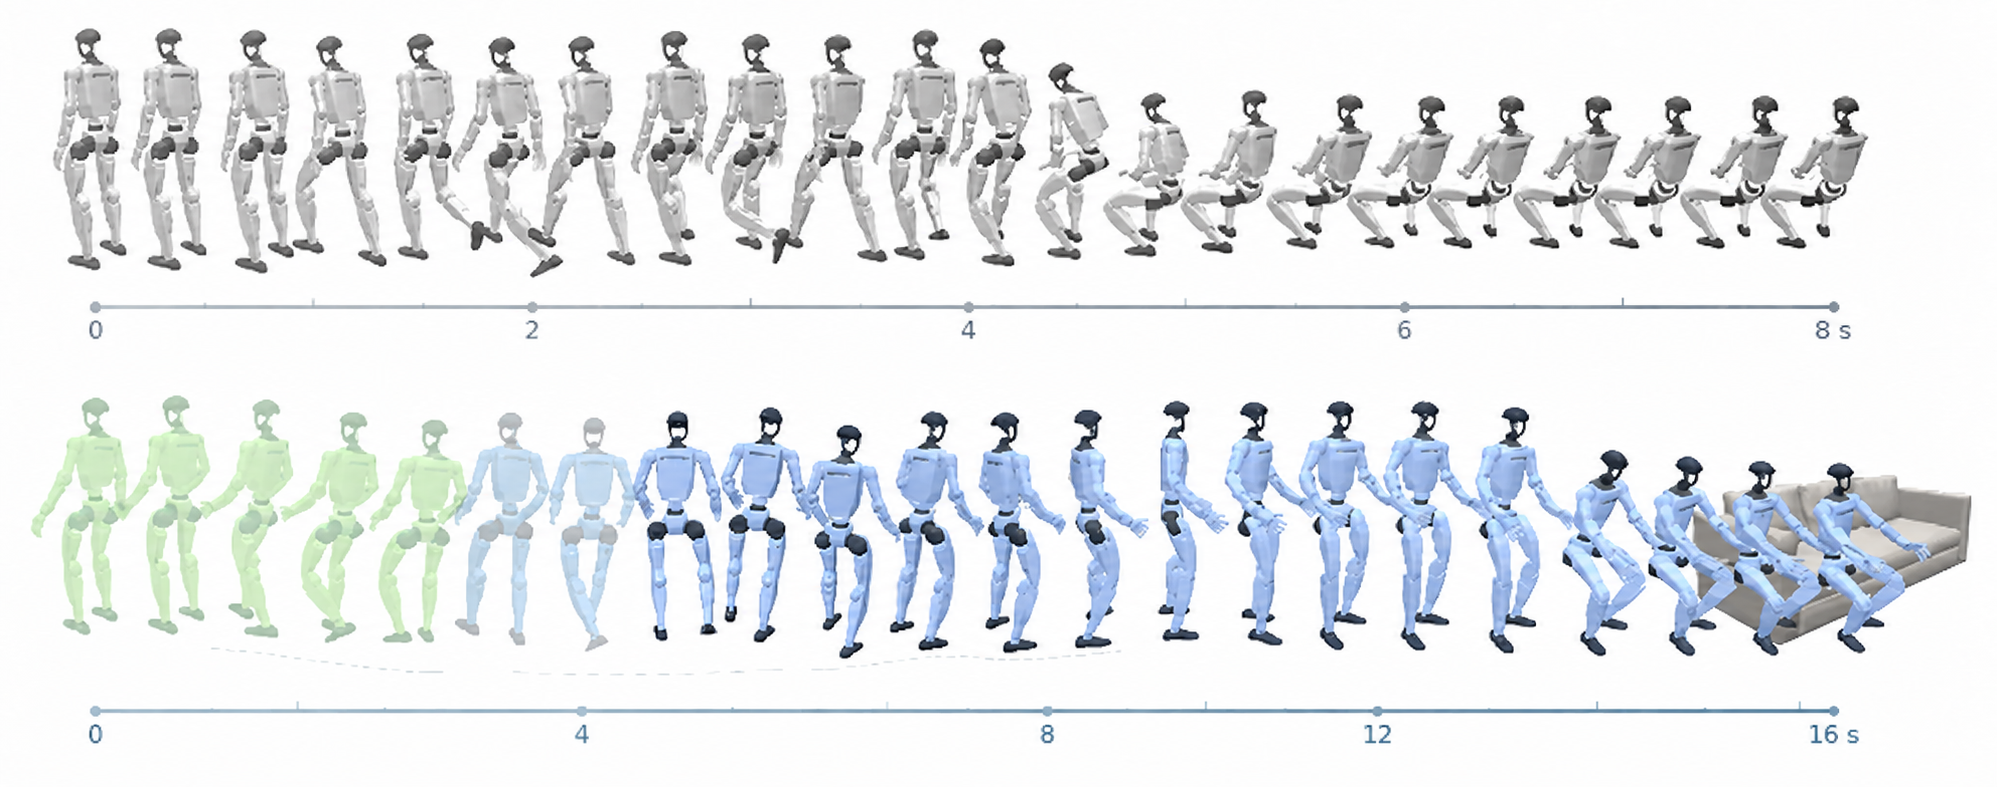
\includegraphics[width=\textwidth]{image/method_2.png}
  \caption{\textbf{Motion-Prior Transfer for Closed-Loop Control.} Top: frozen Kimodo generates a complete ``Sit on the sofa'' sequence from text alone. Bottom: Kimodo-Policy grounds the same prior with visual observations and motion history, repeatedly predicting short chunks for closed-loop execution. Light brown denotes observed history; blue denotes predicted and executed motion.}
  \label{fig:t2m_transfer}
\end{figure}

\textbf{Motion-History Conditioning.} T2M models generate extended motion sequences, whereas closed-loop policies repeatedly predict short action chunks, execute a prefix, and replan from new observations. A fixed sequence cannot accommodate deviations between predicted and measured motion or changes in the scene. We bridge this temporal mismatch by treating each query as constrained motion completion in Kimodo's kinematic representation. Observed history occupies the prefix of a history--future window, with a feature-wise mask identifying available kinematic values. The prefix is restored before each denoising step, while the unconstrained future is generated as the next action chunk. Trainable ControlNet branches inject current egocentric image features into Kimodo's root and body denoisers, grounding predictions in the scene while preserving the pretrained root--body structure. The motion tracker executes a prefix of the chunk; updated state history and images then condition the next prediction. This receding-horizon formulation preserves the structured motion prior while enabling continual visual and state-based correction.

\subsection{Training and Inference}
\label{sec:training_inference}

\textbf{Training Objective.} ControlNet branches and HandNet learn by denoising demonstration windows. At sampled diffusion timesteps, Gaussian noise perturbs normalized root--body features and hand targets; feature-wise masks constrain observed history, with supervision on valid future frames:
\begin{equation}
  \mathcal{L}=\lambda_r\mathcal{L}_{r}+\lambda_b\mathcal{L}_{b}
  +\lambda_h\bigl(\mathcal{L}_{h}+\lambda_{\Delta}\mathcal{L}_{\Delta}\bigr),
  \label{eq:policy_training_objective}
\end{equation}
The masked MSE terms $\mathcal{L}_{r}$, $\mathcal{L}_{b}$, and $\mathcal{L}_{h}$ reconstruct clean normalized root--body features and hand targets. Binary hand targets use $[-1,1]$; continuous targets are closure residuals relative to the latest valid observed hand state. $\mathcal{L}_{\Delta}$ measures $\ell_1$ error between predicted and demonstrated consecutive hand-control changes, including the observed-to-first-future transition; continuous residuals are first converted to closure values. Motion and hand losses mask padding; hand losses also mask unavailable labels, and transition terms require two valid adjacent labels. The main MSE configuration uses $(\lambda_r,\lambda_b,\lambda_h,\lambda_{\Delta})=(4,1,1,0.2)$. Predicted root motion and, in the main configuration, root ControlNet features are detached before body generation; HandNet receives detached body and visual features. The Kimodo denoisers and DINOv3~\cite{dinov3} encoder remain frozen.

\textbf{Inference.} At each policy query, we encode the language instruction and current egocentric image, and represent the available proprioceptive history in Kimodo's motion space with frame- and feature-wise observation masks. We initialize the future motion and hand sequences from Gaussian noise and iteratively denoise them with DDIM~\cite{song2022denoisingdiffusionimplicitmodels}. At each step, the observed history is restored, visual features are injected into the frozen root and body denoisers through ControlNet, the predicted root conditions body generation, and HandNet predicts hand controls from the current hand state, visual features, and future body features. After the final denoising step, we invert the motion representation and map the resulting root and joint trajectories, together with bilateral hand commands, to tracker-compatible references. The low-level whole-body tracker executes a chunk prefix; the policy replans from updated visual observations and proprioceptive states. This receding-horizon loop combines structured motion generation with continual closed-loop correction.
